\lab{Algorithms}{Introduction to Wavelets}{Intro to Wavelets}

\objective{This section explains the basic ideas of Wavelet Analysis
using the Haar wavelet as a prototypical example.}

Recall that in the context of Fourier analysis, one seeks to represent a
function in the frequency domain, and this is accomplished via the Fourier
transform. The Fourier transform allows us to analyze and process functions
in many useful ways, as you have seen in previous labs. There are, however,
drawbacks to this approach. For example, although a function's Fourier
transform gives us complete information on its frequency spectrum, time
information is lost. We can know which frequencies are the
most prevalent, but not when they occur. This is due in part to the fact that
the sinusoidal function $f(x) = e^{2\pi ix}$ -- on which the Fourier transform
is based -- has infinite support. Its nature is essentially \emph{non-local},
and so the Fourier transform fails to provide local information in both the
time and frequency domains. This brings us to the following question: are
there types of transforms that avoid the shortcomings mentioned above? The
answer is an emphatic yes. Enter Wavelet analysis.

\section*{The Haar Wavelet}

As noted earlier, the Fourier transform is based on the complex exponential
function. Let us alter the situation and consider instead the following
function, known as the \emph{Haar wavelet}:
\begin{equation*}
\psi(x) =
 \begin{cases}
  1 & \text{if } 0 \leq x < \frac{1}{2} \\
  -1 & \text{if } \frac{1}{2} \leq x < 1 \\
  0 & \text{otherwise.}
 \end{cases}
\end{equation*}

% It might be nice to plot this function and include the image in the lab.

Along with this wavelet, we introduce the associated \emph{scaling function}:
\begin{equation*}
\phi(x) =
 \begin{cases}
 1 & \text{if } 0 \leq x < 1 \\
 0 & \text{otherwise.}
 \end{cases}
\end{equation*}

From the wavelet and scaling function, we can generate two countable families
of dyadic dilates and translates given by
\begin{equation*}
\psi_{m,k}(x) = \psi(2^mx - k)
\end{equation*}
\begin{equation*}
\phi_{m,k}(x) = \phi(2^mx - k),
\end{equation*}
where $m,k \in \mathbb{Z}$.

Let us focus for the moment on that second family of functions, $\{\phi_{m,k}\}$.
If we fix $m$ and let $k$ vary over the integers, we have a countable collection of
simple functions. The support of a typical function $\phi_{m,k}$ is the interval
$[k2^{-m}, (k+1)2^{-m}]$, and for any $m \in \mathbb{Z}$ we have
\begin{equation*}
\mathbb{R} = \displaystyle\biguplus_k\,[k2^{-m}, (k+1)2^{-m}],
\end{equation*}
where $\uplus$ denotes a union over disjoint sets. Thus, the supports can be viewed as
a discretization of the real line, and we can use this collection of simple functions
to approximate any $f \in L^2(\mathbb{R})$ in the following sense:
\begin{equation*}
f(x) \approx f_m(x) := \displaystyle\sum_{k \in \mathbb{Z}}\alpha_{m,k}\phi_{m,k}(x),
\end{equation*}
where
\begin{equation*}
\alpha_{m,k} := 2^m \displaystyle \int_{k2^{-m}}^{(k+1)2^{-m}}f(x) dx
\end{equation*}
($\alpha_{m,k}$ is simply the average value of $f$ on $[k2^{-m},(k+1)2^{-m}]$). As you
would probably expect, the point-wise error between $f$ and its approximation $f_m$
(called a \emph{frame}) goes to zero as $m \to \infty$.

These frames are not quite good enough, however. Each coefficient $\alpha_{m,k}$
certainly captures local information about $f$ -- namely its average value on
a certain interval -- but it fails to tell us anything about how $f$ changes
on that interval. We need more information than is provided by $f_m$ in order
to know about discontinuities or high-frequency oscillations of $f$. To this end,
we now consider the wavelet function $\psi$.
Notice that the Haar wavelet is oscillatory in nature, and is thus better suited
to capture local information on how a function changes at a given point. For
any given $m$, we define a function $d_m$, called a \emph{detail}, as follows:
\begin{equation*}
d_m(x) := \displaystyle\sum_{k \in \mathbb{Z}}\beta_{m,k}\psi_{m,k}(x),
\end{equation*}
where
\begin{equation*}
\beta_{m,k} := 2^m \displaystyle \int_{-\infty}^{\infty}f(x) \psi_{m,k}(x) dx.
\end{equation*}
Each coefficient $\beta_{m,k}$ gives information about how $f$ changes on the
the interval $[k2^{-m}, (k+1)2^{-m}]$, and larger coefficients correspond
to larger spikes of width $2^{-m}$. Thus, as $m$ increases, the
detail function $d_m$ gives information about the higher-frequency oscillations
of the function. The details and approximation frames interact in the following way:
\begin{equation*}
f_{m+1} = f_m + d_m.
\end{equation*}
As a result of this fortuitous relationship, one can prove the decomposition
\begin{equation*}
L^2(R) = V_0 \oplus W_0 \oplus W_1 \oplus \cdots,
\end{equation*}
where $V_j := \text{span}\{\phi_{j,k}\}_{k \in \mathbb{Z}}$ and
$W_j := \text{span}\{\psi_{j,k}\}_{k \in \mathbb{Z}}$. This fact justifies
our hope to approximate and analyze functions using wavelets.
\begin{figure}[t]
\minipage{0.32\textwidth}
    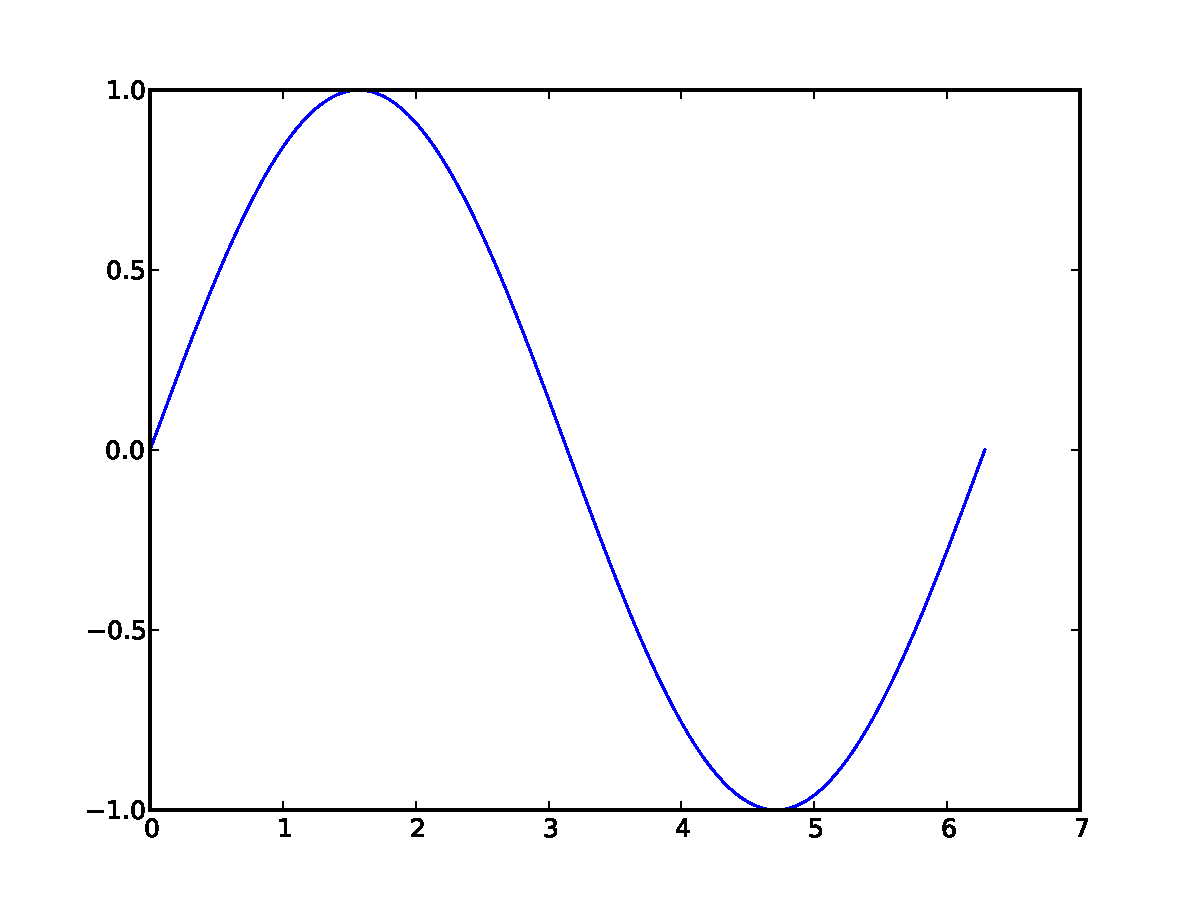
\includegraphics[width=\linewidth]{sinecurve}
    \caption{$f(x) = \sin (x)$}
\endminipage\hfill
\minipage{0.32\textwidth}
    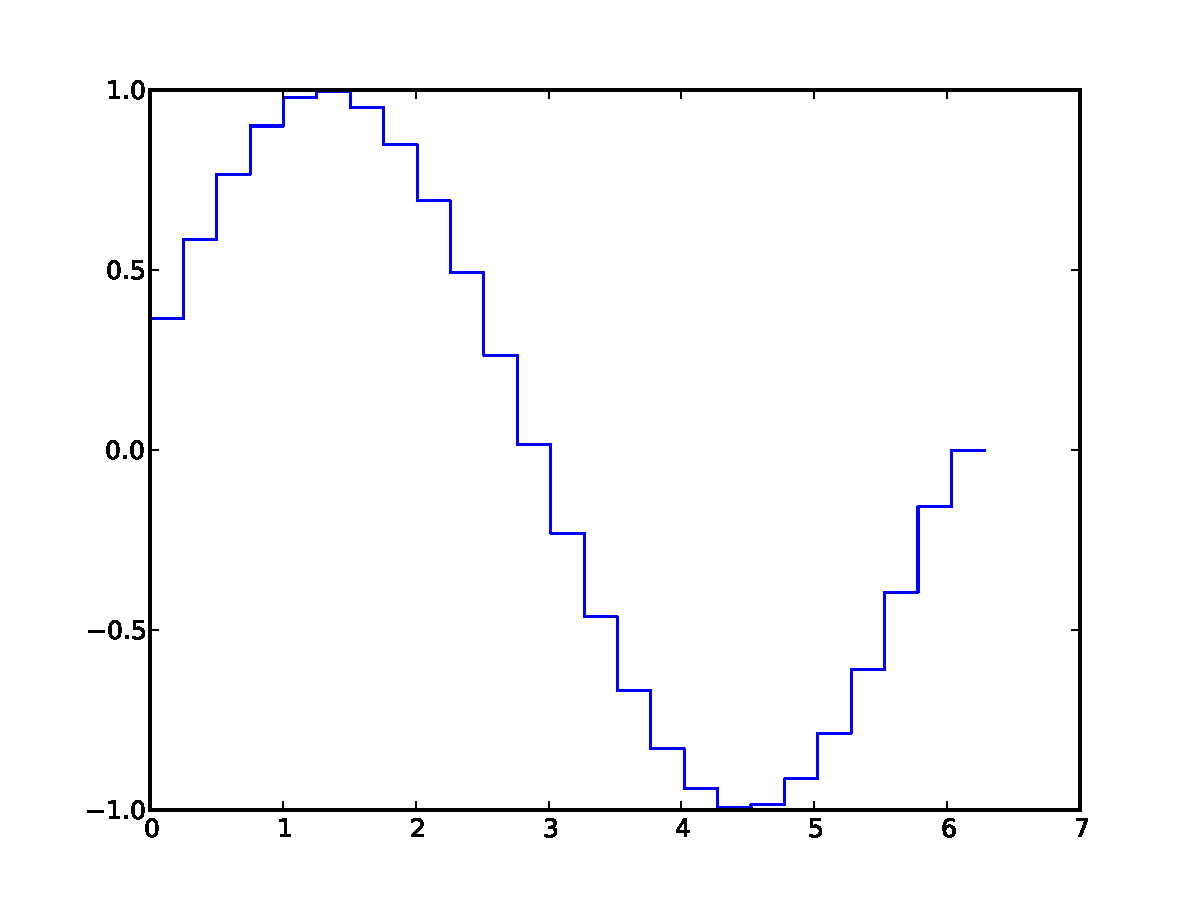
\includegraphics[width=\linewidth]{discreteSineCurve.pdf}
    \caption{$f_4$}
\endminipage\hfill
\minipage{0.32\textwidth}
    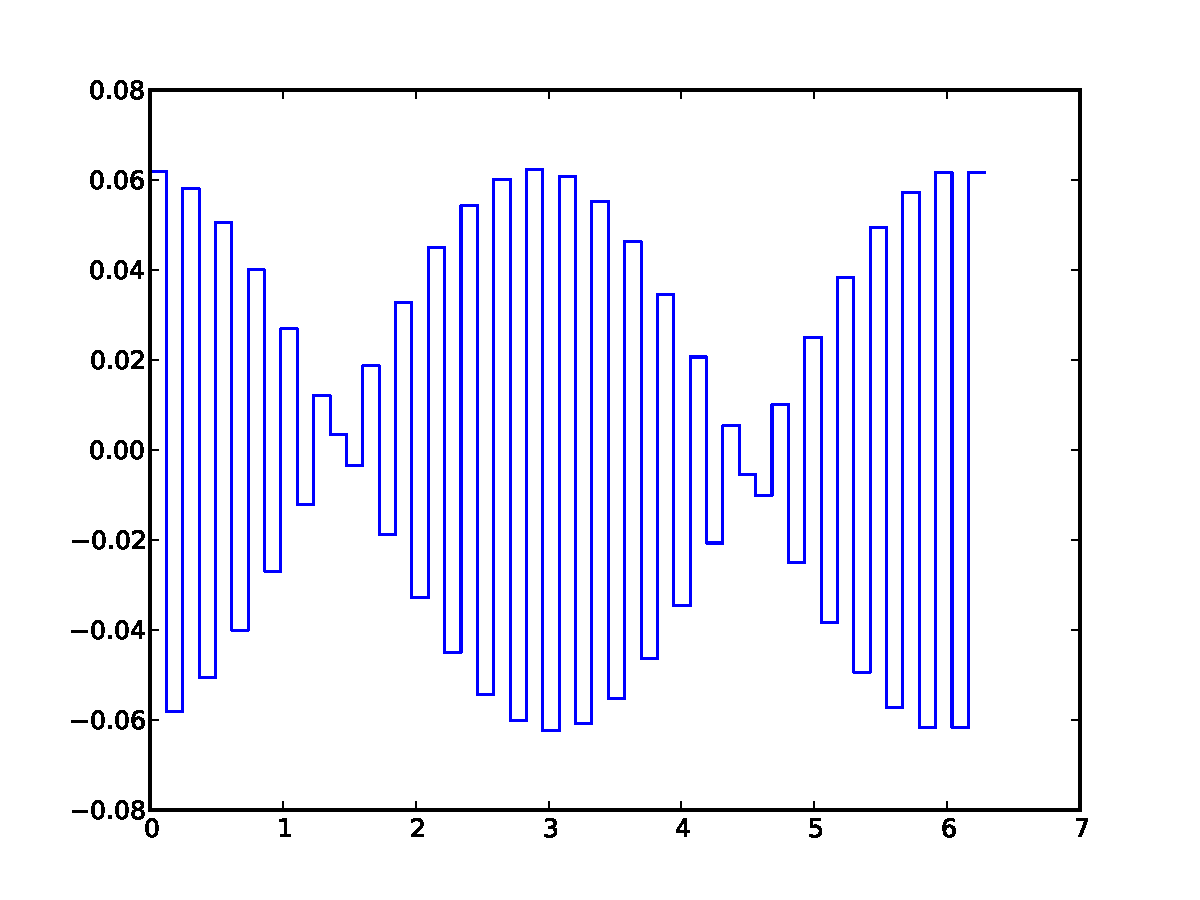
\includegraphics[width=\linewidth]{sineCurveDetail}
    \caption{$d_4$}
\endminipage
\end{figure}
\begin{problem}
Calculate and plot the approximation frames for $f(x) = \sin(x)$ on the interval $[0,2\pi]$
for $m = 4, 6, 8$. Note that because we are working on a finite interval,
we only need to calculate certain coefficients $\alpha_{m,k}$. In
particular, we only need the coefficients for $k = 0$ up to the first integer
$n$ such that $(n+1)2^{-m} > 2 \pi$ (why?). Furthermore, to plot the frame,
all we need is an array containing the relevant coefficients. Then simply plot
the coefficients against \li{linspace} with appropriate arguments
and set \li{drawstyle='steps'} in the \li{plt.plot} function.
\end{problem}

\begin{problem}
Now calculate the details for $f(x) = \sin(x)$ on the same interval and for the
same $m$ values given above. Use previous results to compute the coefficients
for $f_5$, $f_7$, and $f_9$ and plot them.
\end{problem}

\section*{The Discrete Wavelet Transform}

What purpose do these details and approximation frames serve? According to the
properties discussed above, we can approximate $L^2$ functions as follows:
\begin{align*}
f \approx f_{J+1} &= f_J + d_J \\
&= f_{J-1} + d_{J-1} + d_J \\
& \ldots\\
&= f_{I} + d_{I} + d_{I+1} + \cdots + d_J,
\end{align*}
where $1 \leq I \leq J$. If $f$ has compact support (as in the case of a finite-time signal,
for example), only finitely many of the coefficients in the frame and the details are
nonzero, thus enabling us to represent $f$ to a reasonable degree of accuracy in a very
efficient manner. The calculation of these detail coefficients is called the \emph{discrete
wavelet transform}. In the context of signals processing, one can imagine calculating these
coefficients, transmitting them, and then reproducing the approximated signal on the
receiving end. Furthermore, the coefficients of the details reflect the local properties
of the original function $f$ at the particular level of detail and resolution! This means
that we can discard many of the coefficients if we are only interested in reproducing a certain
part of the signal, or in recovering the entire signal to only a limited resolution. We can
also study just those frequencies of the signal that fall within a certain range (called a
sub-band) by examining the detail coefficients at a particular level. These
properties make the discrete wavelet transform an attractive alternative to the Fourier
transform in many applications.

In practice, we are often interested in analyzing discrete signals with compact support (that is,
finite-time signals that we have sampled at a finite number of points). If wavelet analysis is
to be of any use, we first need an efficient way to calculate the discrete wavelet transform.
The process described in the first section, while intuitive and illustrative of the mathematical
principles
behind wavelet analysis, is not the best approach to calculating the wavelet coefficients. It
turns out that the discrete wavelet transform can be implemented as an iterated low-pass/high-
pass filter bank, one iteration of which is shown graphically in the figure. We present the
algorithm without getting into the details of why it works.
\begin{figure}[H]
\centering
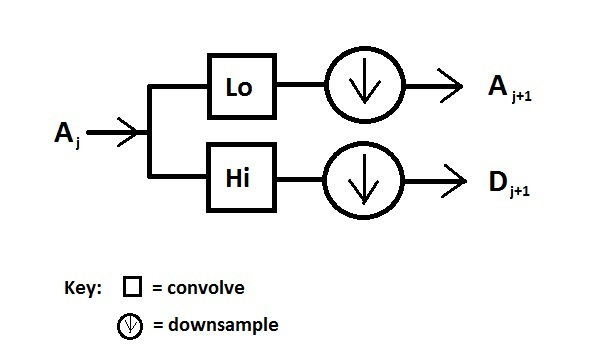
\includegraphics[width = 0.5\textwidth]{dwt1}
\caption{The one-dimensional discrete wavelet transform.}
\end{figure}
The input, $A_j$, represents the level-$j$ approximation frame, and we initialize $A_0$ to
simply be the original signal. Lo and Hi are the low-pass and high-pass filters, respectively.
(By \emph{filter} we mean a vector that serves the purpose of extracting or suppressing a
particular feature of the signal. The Lo and Hi filters are obtained from the wavelet at hand;
for the Haar wavelet, Lo $= (\sqrt{2}^{-1}, \sqrt{2}^{-1})$ and Hi $= (-\sqrt{2}^{-1}, \sqrt{2}
^{-1})$.) The box means convolve the input with the filter, and the circle means downsample by
a factor of two, i.e. remove either the even or odd-indexed entries of the input. The outputs,
$A_{j+1}$ and $D_{j+1}$, are the level-$(j+1)$ approximation frame and detail coefficients,
respectively. Note that the length of the input array is twice that of the output arrays. The
detail coefficients $D_{j+1}$ are stored, and $A_{j+1}$ is then fed back into the loop. Continue
this process until the length of the output is less than the length of the filters, and
return all of the stored detail coefficients as well as the final approximation frame.
\begin{problem}
Write a function that calculates the discrete wavelet transform as described above.
The inputs should be three one-dimensional NumPy arrays (the signal, low-pass filter, and
high-pass filter). The output should be a list of one-dimensional NumPy arrays in the
following form: $[A_n, D_n, D_{n-1},\ldots,D_1]$. (Note: for the convolution, you may use
the \li{fftconvolve} function from the \li{scipy.signal} package using the default
\li{mode = 'full'} parameter, but note that the output array is one entry too large, and so
you need to omit the first entry. For downsampling, only keep the even-indexed entries.)
\end{problem}
We also need to know how to reconstruct the signal from the detail coefficients and
approximation frame. Fortunately, the algorithm described above is entirely reversible,
albeit with slightly different filters: Lo $= (\sqrt{2}^{-1}, \sqrt{2}^{-1})$ and
Hi $= (\sqrt{2}^{-1}, -\sqrt{2}^{-1})$.
Given $A_{j+1}$ and $D_{j+1}$, simply upsample both arrays (by inserting a zero after
each entry of the original array), convolve the results
with the Lo and Hi filters, respectively (this time omit the \emph{last} entry of the
result), and add the outputs to obtain $A_j$. Continue the
process until you recover $A_0$, the original signal.
\begin{problem}
Write a function that calculates the inverse wavelet transform as described above.
The inputs should be a list of arrays (of the same form as the output of your discrete
wavelet transform function), the low-pass filter, and the high-pass filter. The output
should be a single array, the recovered signal. In order to check your work, compute
the discrete wavelet transform of a random array of length 64, then compute the inverse
transform, and compare the original signal with the recovered signal. The difference
should be very small.
\end{problem}

\section*{More Wavelets}
Up to this point, the only wavelet that we have considered is the Haar wavelet, 
which is the simplest and historically first example. Wavelet analysis is a broad 
field, however, and there are myriad other wavelets that have been studied and 
applied. Your implementation of the discrete wavelet transform is quite general, 
and you will find that different types of signals or functions call for different 
wavelets. We will not go into detail here, but be aware that there is a large 
selection of wavelets out there. 

\begin{figure}[H]
\minipage{0.49\textwidth}
    \includegraphics[width=\linewidth]{mexicanHat}
    \caption{The Mexican Hat Wavelet}
\endminipage\hfill
\minipage{0.49\textwidth}
    \includegraphics[width=\linewidth]{db5_3}
    \caption{The Cohen-Daubechies-Feauveau 5/3 Wavelet}
\endminipage
\end{figure}